\documentclass[12pt,a4paper]{article}

\setlength{\textwidth}{165mm}
\setlength{\textheight}{240mm}
\setlength{\parindent}{0mm} % S{\aa} meget rykkes ind efter afsnit
\setlength{\parskip}{\parsep}
\setlength{\headheight}{0mm}
\setlength{\headsep}{0mm}
\setlength{\hoffset}{-2.5mm}
\setlength{\voffset}{0mm}
\setlength{\footskip}{15mm}
\setlength{\oddsidemargin}{0mm}
\setlength{\topmargin}{0mm}
\setlength{\evensidemargin}{0mm}

\usepackage[all]{xy}
\usepackage{graphicx}    % For grafik (billederfiler)
\usepackage[T1]{fontenc} % For at blande \textsc{} med \textbf{}
\usepackage[utf8]{inputenc}
\usepackage{amsfonts,amsmath,amssymb}
\usepackage{eucal}
\usepackage[danish]{babel}
\usepackage{enumerate}  
\usepackage{hyperref}
\usepackage{url}
\usepackage{mathptmx}
\usepackage{multirow}
\usepackage[dvipsnames,usenames]{color}
\usepackage{tabularx,colortbl,xcolor}
\usepackage{listings}
\usepackage{color}
\usepackage{amsmath}
\usepackage{xcolor}

\definecolor{KU-red}{RGB}{144,26,30} 
\definecolor{dkgreen}{rgb}{0,0.6,0}
\definecolor{gray}{rgb}{0.5,0.5,0.5}
\definecolor{mauve}{rgb}{0.58,0,0.82}

\lstset{frame=tb,
  language=Java,
  aboveskip=3mm,
  belowskip=3mm,
  showstringspaces=false,
  columns=flexible,
  basicstyle={\small\ttfamily},
  numbers=none,
  numberstyle=\tiny\color{gray},
  keywordstyle=\color{blue},
  commentstyle=\color{dkgreen},
  stringstyle=\color{mauve},
  breaklines=true,
  breakatwhitespace=true,
  tabsize=3}

\DeclareSymbolFont{usualmathcal}{OMS}{cmsy}{m}{n}
\DeclareSymbolFontAlphabet{\mathcal}{usualmathcal}
\DeclareSymbolFont{letters}{OML}{txmi}{m}{it}

\DeclareMathSymbol{\alpha}{\mathord}{letters}{"0B}
\DeclareMathSymbol{\beta}{\mathord}{letters}{"0C}
\DeclareMathSymbol{\gamma}{\mathord}{letters}{"0D}
\DeclareMathSymbol{\delta}{\mathord}{letters}{"0E}
\DeclareMathSymbol{\epsilon}{\mathord}{letters}{"0F}
\DeclareMathSymbol{\zeta}{\mathord}{letters}{"10}
\DeclareMathSymbol{\eta}{\mathord}{letters}{"11}
\DeclareMathSymbol{\theta}{\mathord}{letters}{"12}
\DeclareMathSymbol{\iota}{\mathord}{letters}{"13}
\DeclareMathSymbol{\kappa}{\mathord}{letters}{"14}
\DeclareMathSymbol{\lambda}{\mathord}{letters}{"15}
\DeclareMathSymbol{\mu}{\mathord}{letters}{"16}
\DeclareMathSymbol{\nu}{\mathord}{letters}{"17}
\DeclareMathSymbol{\xi}{\mathord}{letters}{"18}
\DeclareMathSymbol{\pi}{\mathord}{letters}{"19}
\DeclareMathSymbol{\rho}{\mathord}{letters}{"1A}
\DeclareMathSymbol{\sigma}{\mathord}{letters}{"1B}
\DeclareMathSymbol{\tau}{\mathord}{letters}{"1C}
\DeclareMathSymbol{\upsilon}{\mathord}{letters}{"1D}
\DeclareMathSymbol{\phi}{\mathord}{letters}{"1E}
\DeclareMathSymbol{\chi}{\mathord}{letters}{"1F}
\DeclareMathSymbol{\psi}{\mathord}{letters}{"20}
\DeclareMathSymbol{\omega}{\mathord}{letters}{"21}
\DeclareMathSymbol{\varepsilon}{\mathord}{letters}{"22}
\DeclareMathSymbol{\vartheta}{\mathord}{letters}{"23}
\DeclareMathSymbol{\varpi}{\mathord}{letters}{"24}
\DeclareMathSymbol{\varrho}{\mathord}{letters}{"25}
\DeclareMathSymbol{\varsigma}{\mathord}{letters}{"26}
\DeclareMathSymbol{\varphi}{\mathord}{letters}{"27}
\DeclareMathSymbol{\Gamma}{\mathord}{letters}{"00}
\DeclareMathSymbol{\Delta}{\mathord}{letters}{"01}
\DeclareMathSymbol{\Theta}{\mathord}{letters}{"02}
\DeclareMathSymbol{\Lambda}{\mathord}{letters}{"03}
\DeclareMathSymbol{\Xi}{\mathord}{letters}{"04}
\DeclareMathSymbol{\Pi}{\mathord}{letters}{"05}
\DeclareMathSymbol{\Sigma}{\mathord}{letters}{"06}
\DeclareMathSymbol{\Upsilon}{\mathord}{letters}{"07}
\DeclareMathSymbol{\Phi}{\mathord}{letters}{"08}
\DeclareMathSymbol{\Psi}{\mathord}{letters}{"09}
\DeclareMathSymbol{\Omega}{\mathord}{letters}{"0A}
\DeclareMathSymbol{\upGamma}{\mathalpha}{operators}{"00}
\DeclareMathSymbol{\upDelta}{\mathalpha}{operators}{"01}
\DeclareMathSymbol{\upTheta}{\mathalpha}{operators}{"02}
\DeclareMathSymbol{\upLambda}{\mathalpha}{operators}{"03}
\DeclareMathSymbol{\upXi}{\mathalpha}{operators}{"04}
\DeclareMathSymbol{\upPi}{\mathalpha}{operators}{"05}
\DeclareMathSymbol{\upSigma}{\mathalpha}{operators}{"06}
\DeclareMathSymbol{\upUpsilon}{\mathalpha}{operators}{"07}
\DeclareMathSymbol{\upPhi}{\mathalpha}{operators}{"08}
\DeclareMathSymbol{\upPsi}{\mathalpha}{operators}{"09}
\DeclareMathSymbol{\upOmega}{\mathalpha}{operators}{"0A}

\newcommand{\hhemail}[1]{\textsf{#1}}
\newcommand{\hhurl}[1]{{\color{blue}\url{#1}}}

\begin{document}
	
	\begin{minipage}[b]{1.0\linewidth} 
		
\includegraphics[height=50mm]{KULogo.pdf}
		
		\vspace*{-16ex}
		\vspace {35ex}
		\begin{center}
			{\huge \bf Project: Beetle} \vspace*{4ex} \\
			{\large 23. march 2014}\\
			\vspace*{2ex}
			qzj710 - 121095 - Enes Golic \\
			rpc308 - 070493 - Yunus Emre Okutan \\
			cbh239 - 250594 - Casper Lützhøft Christensen \\
			mhb558 - 250795 - Tor-Salve Dalsgaard\\
			\vspace*{1ex}
			Instructor - Casper Passau
			
		\end{center}
	\end{minipage}
	
\newpage
\section{Project definition}
Our client is the University of Hamburg – more specifically - their entomology $($insect$)$ department.\\
Due to the university’s agreement with the German government, in order to receive funds in support, the university’s material must be publicly accessible. For that purpose, we must design a search engine and corresponding database, which will be accessible from their website. This will allow people to access the information stored by searching for it and subsequently allow the administrators to add new entries.\\ 

\subsection{Problem statement}
Part one of the project in simple terms is that we have to create a database containing entries that represent insects. An insect in this instance will contain four attributes by which it is characterised: Its name, family, species and genus. Furthermore, each entry must also contain a link to a www.zoomify.com image of the insect. The usage of zoomify is at the request of the university. This is because it allows high-resolution images in which the users can zoom, but also because it prevents a user from simply downloading the image and copying the database. \\
Part two is then creating a search engine affiliated with the database we established. The search engine must allow the user to search for the name of any of the four attributes of an insect in the database. Once the search is finished, the engine must then display all entries that contain an attribute fitting the search-criteria.\\
Part three - the final part – is developing a method, which will allow the employees in the entomology department to both input their own entries into the database we developed and also remove existing entries. This functionality must also be restricted for anybody but the authorised employees, to ensure that the database is only editable by the desired people.\\\\
For the purpose of organising, the functional requirements of the program are:
\begin{itemize}
	\item The program must return any and every entry that contains an attribute that matches the search input
	\item The database must allow the creation of new entries, editing of existing entries and deletion of existing entries
	\item The database must be unable to be edited by anyone save the authorised employees
\end{itemize}
	The non-functional requirements are:\\
\begin{itemize}
	\item The search engine must be developed in PHP so it can run on their website in a standard browser with no additional requirements (plugins etc.)
	\item The method of editing the database must be simple enough for people without pre-existing IT skills to use it.
\end{itemize}

\subsection{Software management plan}
The database part of the program, responsible for holding all the data for our client, is to be developed in Oracle SQL using Oracle SQL developer.\\
Proceeding that, the database will communicate with a front-end website containing the search engine, which is to be created using a combination of HTML and CSS for the layout of the website and PHP for the search engine itself.\\
After that, the method which will allow the authorised employees to edit the database. This will be designed according to the client’s specific wishes with their convenience in mind, and will be developed as either a Java-program if they wish to keep it separate from the website or in PHP if they wish it integrated.\\
Naturally we’ll cooperate internally in the group, but for the purpose of ensuring utmost quality-control in all aspects of the development, each necessary part of the process has been given a person of responsibility that will ensure that each respective part functions exactly as desired by the client and intended by us.
In order to assign the right people responsibility for the appropriate tasks, a skill-matrix was developed:\\

\begin{center}
Figure 1: Skill-matrix
\end{center}

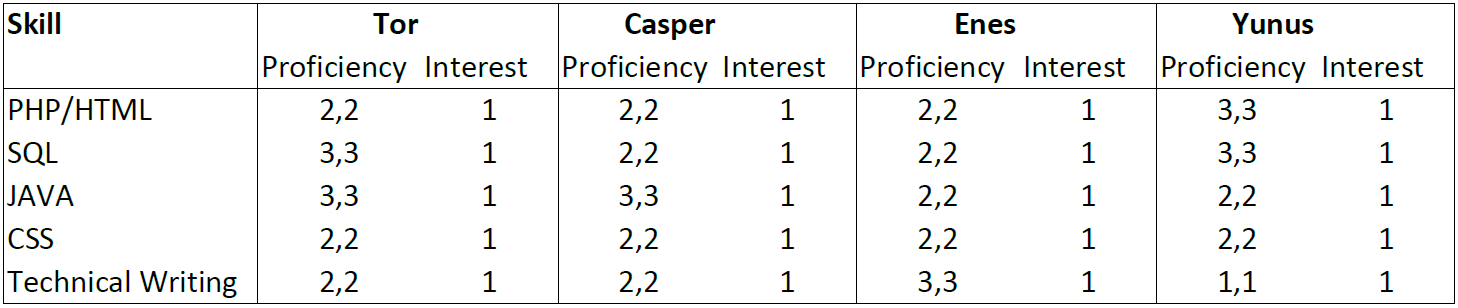
\includegraphics[height=35mm]{Skillmatrix.png}\\

The matrix first of allrepresents a group member's profiency in the skills necessary for the completition of our product, expressed by a tuple $($x,y$)$ where X is a value from 1 to 3 and represents the member's capability relative to the course material.\\
A 1 for instance would imply difficulties, a 2 meets the course's demands and a 3 goes above and beyond what has been taught.\\
The Y, also a value from 1 to 3, represents the degree to which work done by the individual member requires supervision/assistance. \\
A 1 here will imply that assistance is required when the skill is used, a 2 implies that the work produced with the represented skill should be looked over by the group for the sake of corrections or improvements, and a 3 means that work can be done with no assistance/supervision from the group whatsoever.\\
In addition to that, we've got an interest-parametre represented by either the value 0 or 1, and represents the group member's willingness to work with the associated skill.

With the skill-matrix created, the necessities of the product had to be established.
\\
\newpage
\begin{center}
	Figure 2: Work Breakdown Structure
	
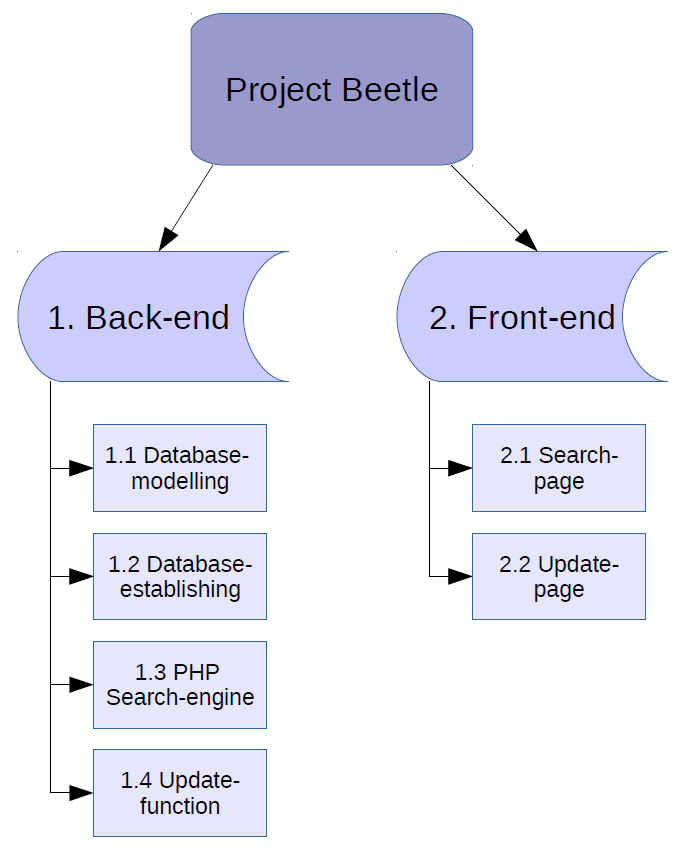
\includegraphics[height=100mm]{WorkBreakdownStructure.png}
\end{center}

On the back-end we will need to model the database and establish it, and and create the search-engine responsible for hopping through the database. Here we'll also need to create the method of updating the database.
On the front-end we'll need to create the website containing the search-engine and also an additional page in which the database can be updated.
Keeping the work-necessities as well as the skill-diagram in mind, different areas of responsibility have been assigned to each individual member of the group.


•	Yunus Emre Okutan – Responsible for development of the search-engine as well as the front-end search-page.\\
•	Enes Golic – Responsible for overall quality-control on the rapport throughout the whole process as well as part of the work on developing the database\\
•	Tor-Salve Dalsgaard – Responsible for ongoing contact with the client and overall managing of the project and, with Enes, responsible for part of the work regarding database development\\
•	Casper Lützhøft Christensen – Responsible for the development of the update-function for allowed parties and also the update-page.

Through succesful breakdown of the work-burden, an approximate scheduling was created depicting the deadlines for parts of the product as well as the necessary hours for completion. This is all showcased in figure 3.
\newpage

\begin{center}
	Figure 3: Scheduling
	
	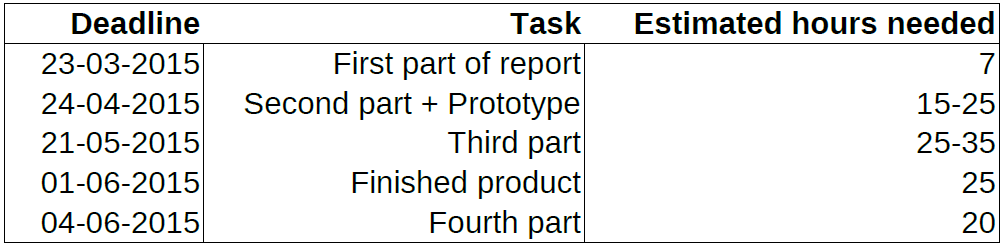
\includegraphics[height=40mm]{Scheduling.png}
\end{center}
In essence, a functional prototype is expected the 24th of April and the finished product the 1st of June.

\subsection{Initial Software Architecture}
\begin{center}
	Figure 4: Software Architecture Diagram
	
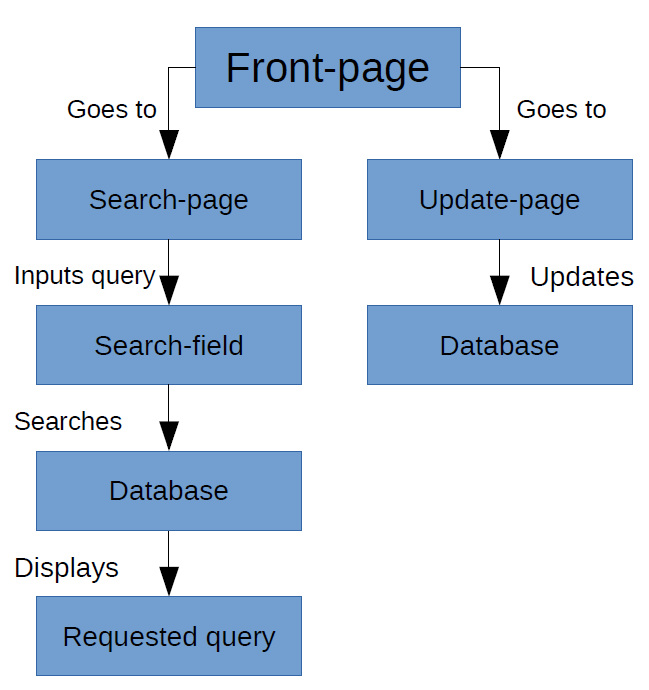
\includegraphics[height=100mm]{SoftwareArchitecture.png}
\end{center}
Figure 3 is a diagram displaying how the different parts of the website's functionality cooperate.
From the front-page either the search-page or the update-page will be visitted.
In the search-page a query can be entered into the search-field, after which the the database will be searched and the results matching the query displayed.
From the update-page, the database can be updated and entries added, edited or removed.	
\newpage
\begin{center}
	Figure 5: Case Diagram
	
	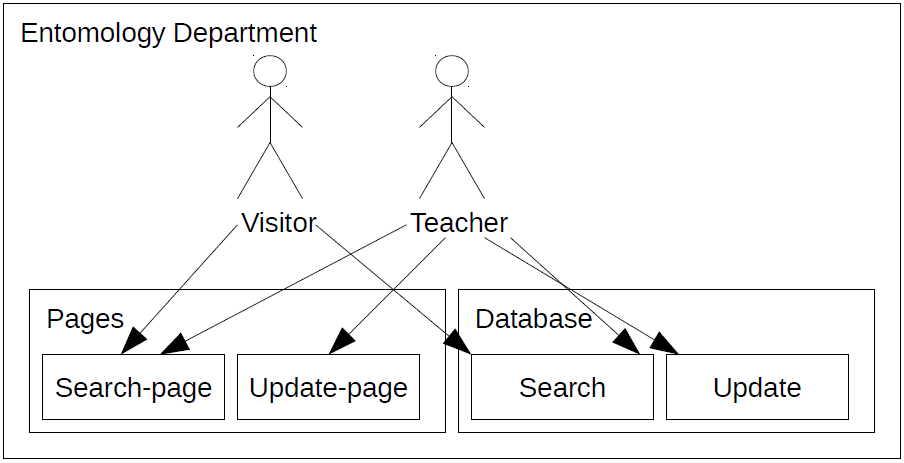
\includegraphics[height=70mm]{CaseDiagram.png}
\end{center}

Figure 4 is a case diagram and depicts the permissions of people potentially visitting the site. 
A normal visitor and a teacher will be able to navigate to the search-page and search the database, but only a teacher will be allowed to navigate to the update-page and update the database.

\newpage
\subsection{Project Agreement Definition}
\textit{Project: Beetle for University of Hamburg developed by Yunus Emre Okutan, Enes Golic, Tor-Salve Dalsgaard and Casper Lützhøft Christensen.}\\

\textbf{Product specification}\\
The product for the University of Hamburg Entomology department will be a database containing entries of insects, a front-end search engine to allow users to search the database and retrieve information and an application to allow the desired employees to edit the database and add, update and remove entries.\\\\
\textbf{Requirements}\\
In order to develop the desired product, we require access to the University of Hamburg’s server so that we can create the database and the search engine on their website. \\
We also require the URLs to all the images of the entries they want added to the database initially, as well as the information corresponding to those.\\\\
\textbf{Payment}\\
The product is being developed as part of the course PKSU from the University of Copenhagen, as such the work committed and product developed are entirely voluntary and no payment is required from the side of the University of Hamburg.\\\\
\textbf{Terms}\\
The University of Hamburg cannot expect a fully functioning product to be delivered; they can however expect our best effort in the endeavor.\\
During development before the final product is delivered, we are in full control of the program and the University of Hamburg must in no way change, delete or in any way modify any parts of the program.\\
Once the product is delivered, it belongs entirely to the University of Hamburg. They are free to use the product for as long as they desire and can freely, in any way modify or delete it if they see fit.\\
We reserve the rights to any methods/code used in the development of the product.\\
All information, knowledge and material that is the property of the University of Hamburg that we encounter during our product-development is entirely confidential and nothing we see or read will ever be exposed to people outside the product agreement.
Given access to the database, we are in no way to edit anything not directly related to the development of our product.\\\\


\_\_\_\_\_\_\_\_\_\_\_\_\_\_\_\_\_\_\_\_ ~~~~~~~~~~~~~\_\_\_\_\_\_\_\_\_\_\_\_\_\_\_\_\_\_\_\_\_\_\_\_\_\_\_\_\_\_\_\_\_\_\_\_\_\_\_\_\_\_\_\_\\
Client~~~~~~~~~~~~~~~~~~~~~~~~~~~~~~~~~~~~~~~~~~~~~Developers       

\newpage
\subsection{Internal Projectetablishment}
The work is set up in the way that people will be focusing on their respective role primarily. Naturally situations will occur where working across these is necessary, but the idea is still to keep people mainly within their assigned area. We expect that each member of the group will spend at least 5 hours every week on their part of the project. In the event that a member of the group is incapable of fulfilling their role due to difficulties/confusion regarding the work, other members of the group will commit to helping the member in question. Should it happen that a member cannot meet his assigned deadline extra work will be assigned due next deadline. In case that member is still unable to fulfill their commitment to the group, internal discussions will be had regarding the responsibilities of said member. \\
The project is to be split into different areas of focus: rapport-writing, coding, database management and, where applicable, leadership and communication. If a change is requested or required it’ll be made through open discussion involving the entirety of the group before the project manager lies down the final verdict.\\
We expect full functionality of the code we write and a rapport without any lacks. We also expect every coding member in the group to be able to pick up new concepts of coding if necessary. Finally, the rapport just as well as the coding is the responsibility of each member in the group, and therefore every member is expected to commit an amount of time and focus to writing parts of the rapport. This is to ensure each member of the group improves their rapport-writing with future writing in mind, but also to ensure maximum quality through different inputs in the group.


                                                   
\end{document}